\begin{center}
  \section{Introduzione all'apparato sperimentale}
\end{center}
\medskip
{\color{gray}\hrule}
\medskip
Quando si sottopone un cristallo semiconduttore a radiazione elettromagnetica nel visibile si osserva che per lunghezze d'onda superiori a un valore critico $\lambda_g$ il materiale si comporta come un buon conduttore ottico, viceversa per lunghezze d'onda inferiori a $\lambda_g$ si comporta come un buon conduttore elettrico. \\
Questo fenomeno deriva dalle proprietà fisiche dei semiconduttori: in questi materiali la differenza di energia tra la banda di valenza (BV) e la banda di conduzione (BC), detta \textit{energy gap}, è compresa tra $0\text{eV}<E_g<3\text{eV}$, valori di energia molto vicini al range di energia trasportata da un fotone nel visibile ($1.8$eV - $3.2$eV). Se l'energia trasportata da un fotone $\frac{hc}{\lambda}$ è minore di $E_g$ allora questa non è sufficiente a promuovere un elettrone nella banda di conduzione e il raggio luminoso attraversa il materiale senza esser assorbito (conducibilità ottica); se $\frac{hc}{\lambda}$ è maggiore di $E_g$, il fotone viene assorbito nel semiconduttore cedendo la sua energia a un elettrone nella BV, il quale salta in BC (conducibitità elettrica).

L'esperienza è dunque volta alla caratterizzazione dell'assorbimento e della trasmissione dell'intensità luminosa $I$ di un campione di Seleniuro di Gallio (GaSe) per poter ricavare tramite successiva analisi una stima del suo \textit{energy gap}.
\subsection{Apparato sperimentale}
\begin{figure}[H]
    \centering
    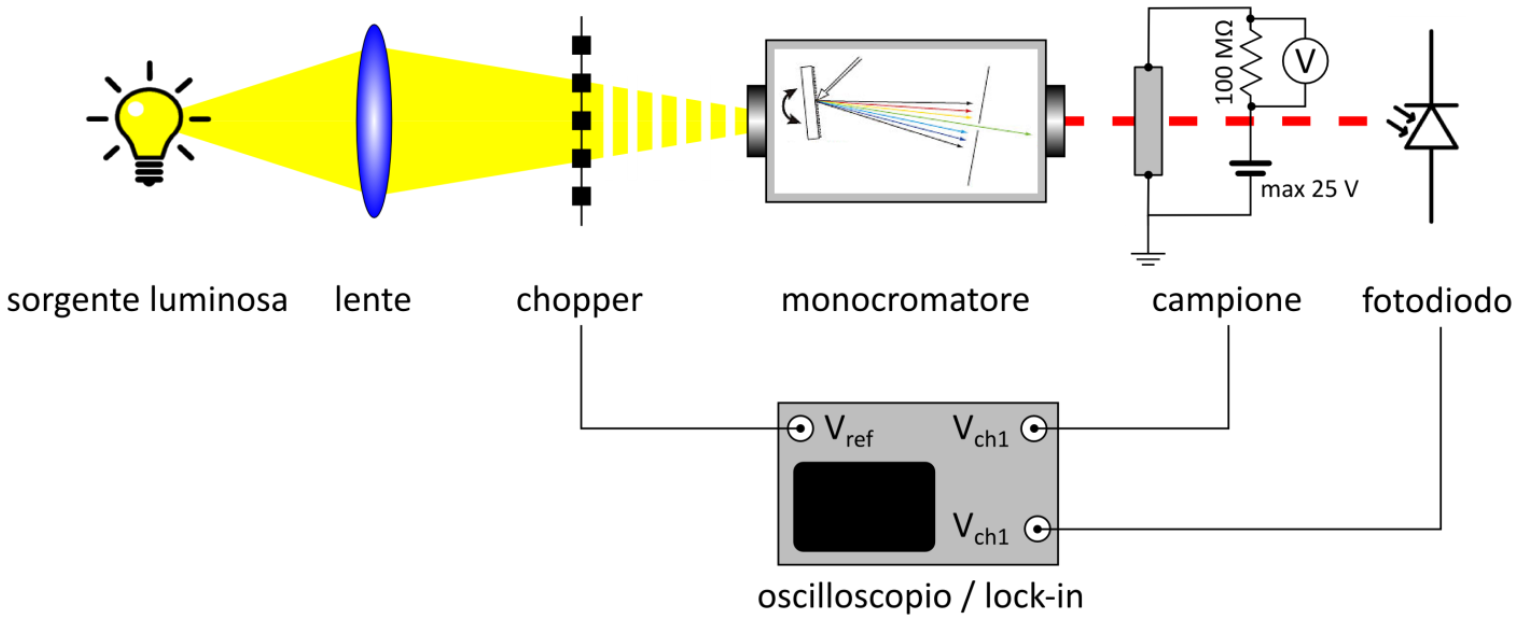
\includegraphics[width=0.77\linewidth]{apparato_sperimentale_fotocond.png}
    \caption{\footnotesize Schema dell'apparato sperimentale.}
    \label{fig:app.sper}
\end{figure}
L'apparato sperimentale principale prevede come sorgente luminosa una lampada a incandescenza, i cui raggi vengono convogliati da una lente all'interno di un monocromatore diffrattivo regolabile tramite una vite micrometrica tarata su una scala arbitraria\footnote{La scala in realtà è una buona approssimazione della lunghezza d'onda selezionata dal monocromatore, tuttavia l'accuratezza della scala è insufficiente per gli scopi dell'esperienza.}. Una fenditura all'uscita del monocromatore permette di filtrare dallo spettro solo una $\Delta \lambda$ sufficientemente piccola da poter essere approssimata a luce monocromatica. Il fascio luminoso monocromatico uscente incide sul campione di SeGa, il quale è fissato su un vetrino e circondato da una montatura metallica per poterlo isolare quanto possibile dalla radiazione ambientale. Infine, lungo l'asse ottico è allineato un fotodiodo grazie al quale è possibile misurare l'intensità luminosa trasmessa dal campione. \\ 
Il campione è inserito all'interno di un circuito elettrico in modo tale da essere in serie ad un generatore di tensione continua - impostato per tutta l'esperienza a $25$V - e a una resistenza di carico di $R_c= (1.00 \pm 0.05)M\Omega$;   poichè la fotocorrente è molto piccola, è inoltre presente un modulo di amplificazione del segnale. Analogamente, il fotodiodo è posto in serie con un generatore di tensione continua e una resistenza di carico. \\ In entrambi i circuiti, la corrente totale è proporzionale all’intensità luminosa assorbita (tenendo conto che una parte della luce incidente viene riflessa); tutte le misure sono state in realtà raccolte sperimentalmente come cadute di potenziale ai capi delle rispettive resistenze di carico e acquisite tramite un oscilloscopio.

\textit{Osservazione} Grazie a un \textit{chopper} (frequenza impostata a $f_{chop}=80$Hz), posto tra la lente e il monocromatore, è stato possibile convertire tutto il segnale da un regime continuo a un regime alternato con frequenza $f_{chop}$. In questo modo è possibile sfruttare un trigger esterno all'oscilloscopio, permettendo a quest'ultimo di leggere solo i segnali con frequenza $f_{chop}$.
\\I segnali di fondo con frequenze diverse da quella del \textit{chopper} non verranno quindi letti, mentre quelli costanti andranno a rappresentare un offset sul segnale armonico.
È particolarmente importante per le misure di fotocorrente in quanto l'ampiezza del segnale è confrontabile con il rumore e se la misura si eseguisse in regime continuo sarebbe difficile distinguere il segnale dal rumore.\\









